\chapter{Method}
\section{Choice of Method}
\begin{figure}[h]
%\hspace*{-0.4cm}
\begin{center}
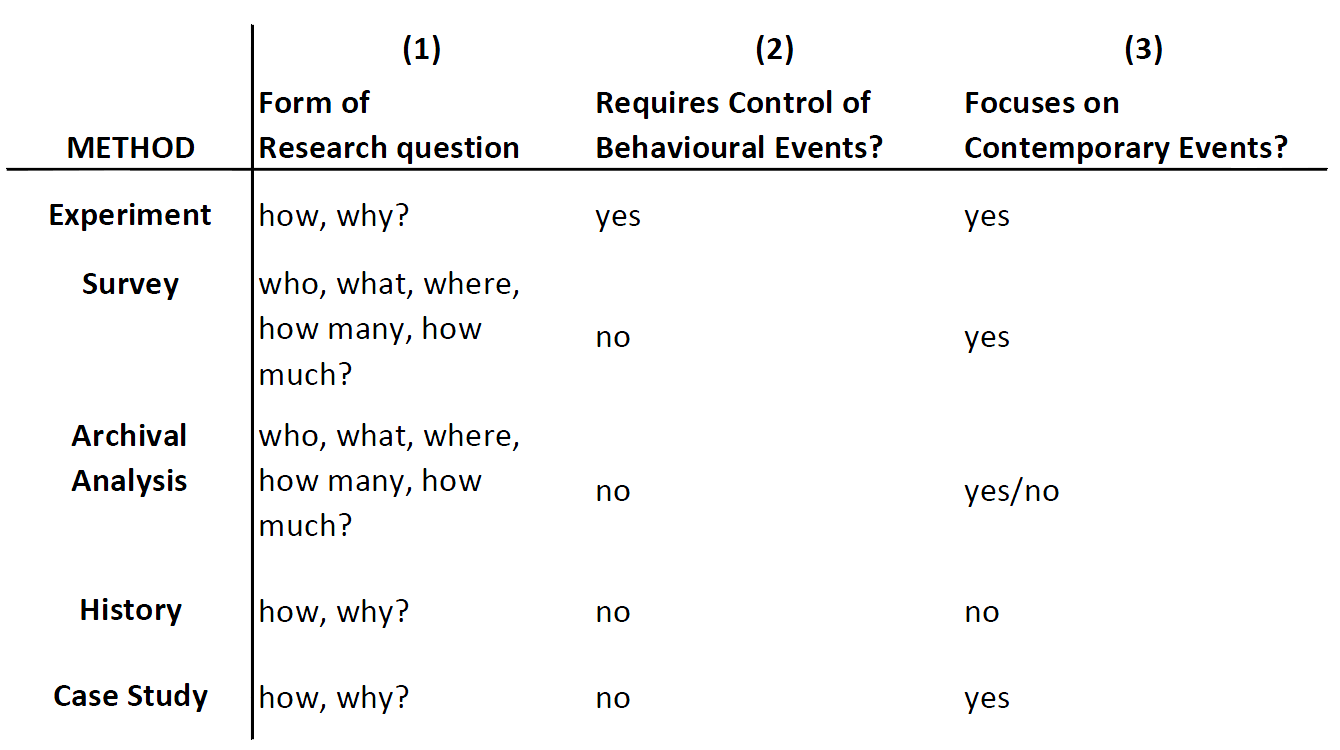
\includegraphics[scale=0.35]{methods.png}
\caption[Situations for different research methods]{Situations for different research methods, derived from \cite{CaseStudyResearch}}
\label{fig:methods}
\end{center}
\end{figure}
\section{Case Study}
%\cite{CaseStudyResearch}
%\cite{kitchenham1995case}
\subsection{Why Case Study?}

\subsection{Background Study}
In order to ask the right questions while interviewing to gathering information for our research, we needed to do thorough background studies of both relevant standards and best practice guidelines. We focused on the accepted international ISO/IEC standards as well as documentation from \ac{NIST}.

We also looked at related work and what has been studied earlier in the field of incident management. 

\subsection{Qualitative research}
The method used in our research is a qualitative method, focusing on relatively few informants. Unlike a quantitative approach typically using questionnaires to gather information from a large number of participants, we aimed for in-depth information gathered from few organizations. This eliminated the possibility to generalize results, but gave us more exhaustive answers and thus better and more suited data for this specific study.

\subsection{Interviews}
Interviews are common and powerful tools to gather information in qualitative research\cite{myers2007qualitative}. We chose to do qualitative instead of quantitative interviews, for the same reasons as stated in the previous section. Cassell and Symon writes \cite{cassell2004essential} that the goal of qualitative interviews is to see the research topic from the interviewee's perspective and understand why and how they got that particular perspective. To meet this goal, qualitative interviews are driven by open questions and a low degree of structure and often focus on specific situations and experiences made by the interviewee.

We wanted the interviewees to talk freely about their experiences, and thus we did not follow a strict list of predefined questions. However, to ensure we got all information required to answer our research questions we used an interview guide. In the interview guide the main goals for our research as well as the main research questions were states along with questions for the interview. They were not followed in strict order, but rather formed the foundation for the dialogue. This gave the opportunity to ask follow-up questions in addition to those predefined. Using an interview guide with some predefined questions and topics is in literature referred to as semi-structured interviews\cite{cassell2004essential}. Due to our inexperience in conducting interviews, the interview guide had some predefined questions(structured), but were still quite open(unstructured). By performing semi-structured interviews, the interviewee can be seen as a ``participant" in the research, rather than an someone only answering pre-defined questions.

The interview guide. 

For this thesis we chose to do face-to-face interviews and to voice recorded the dialogue. 
By conducting interviews face-to-face we could build trust with the interviewee and thus get better and more elaborative answers. It also gave us the opportunity to explain and elaborate on questions that were unclear. Since we recorded all of the interviews we could focus on the listening and thus asking the best follow-up question instead of being extracted by writing answers down. Also, we could listen to the recordings several times as needed and clarify things that were unclear later.

%advantages
\paragraph{Flexible} By choosing this method

%disadvantages
\paragraph{Time-Consuming} Developing an interview guide, carrying out interviews and analysing them can be highly time-consuming activities. Participating in interviews is also time-consuming for interviewees, which could make it challenging to recruit interviewees for our study. One approach to mitigate the risk of not recruiting interviewees for our study was sending out letters explaining the main purpose of the study, what was expected by the interviewee, and how the interviews would play out. We also notified organizations at an early stage and set dates for the interviews to ensure their commitment.


\subsection{Participants}
In the nature of qualitative research participants were chosen to be diverse such that different perspectives on incident management (in the same context) could be studied.
large organizations that are likely to have experiences severe security incidents. + de i gjørvik gjorde på small/medium.. her gjør vi en dybdestudie av noe annet!

Hvorfor de vi valgte?

\paragraph{Practical issues}
\subsection{Document study}
%\subsection{Action Research}
\section{Ethical Considerations}
%Litt i forhold til at man behandler sensitiv information og sånn
\subsection{Anonymization}
\section{Challenges}

